\begin{figure}[h!]
\centering
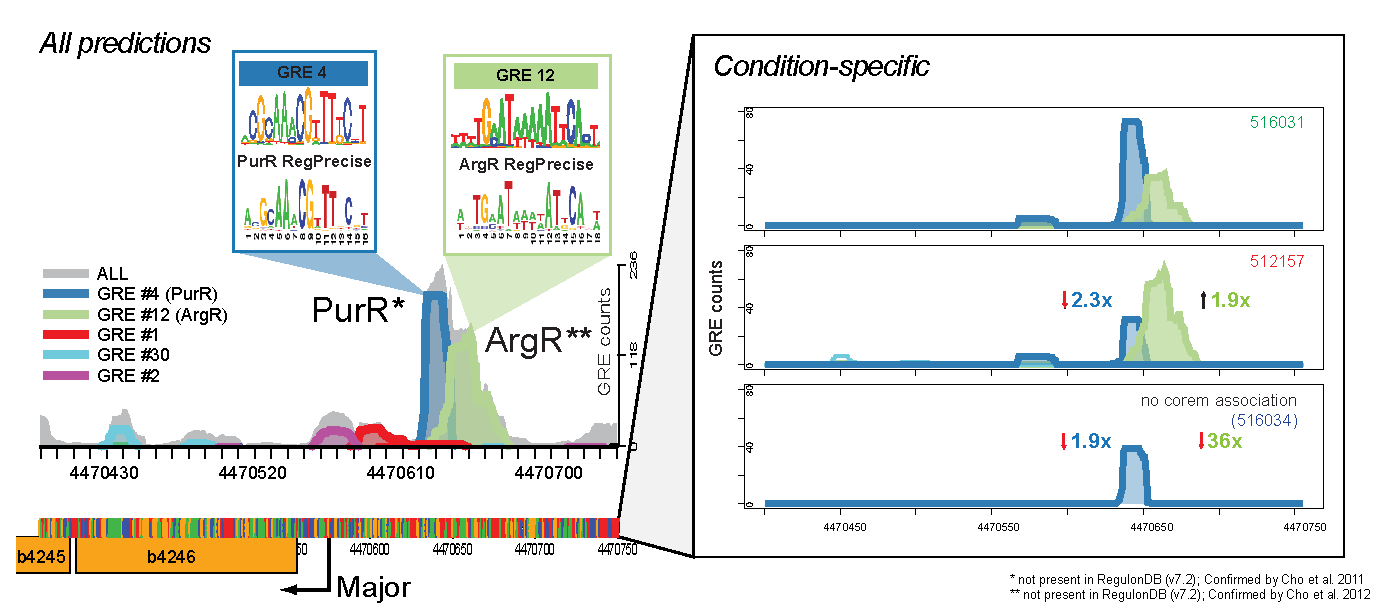
\includegraphics[width=0.95\linewidth]{figures/pyrL.pdf}
\caption[Differential GRE activity in \textit{pyrL} promoter, \textit{E. coli}]{\textbf{Differential GRE activity in \textit{pyrL} promoter, \textit{E. coli}.} (Left) Predicted promoter architecture for {\it E. coli} \textit{pyrL} (\textit{b4246}). Overlapping GREs matching to PurR (GRE \#4) and ArgR (GRE \#12) were detected upstream of pyrL. These sites were not annotated in \rdb, but were validated in independent ChIP-chip experiments \cite{Cho2012,Cho2011a}. Transcription start site indicated with arrow. (Bottom) Condition-specific promoter architectures for {\it E. coli} \textit{pyrL} (as in Figure 2E). Variation in predicted GRE activity across three different subsets of experimental conditions (counts and fold-change) for two GREs in the \textit{pyrL} promoter. Experimental subsets correspond to conditions under which at least one of three nucleotide biosynthetic corems is regulated (denoted by colored names at top-right of each plot)}
\label{fig:pyrL}
\end{figure}

\begin{figure}[h!]
\centering
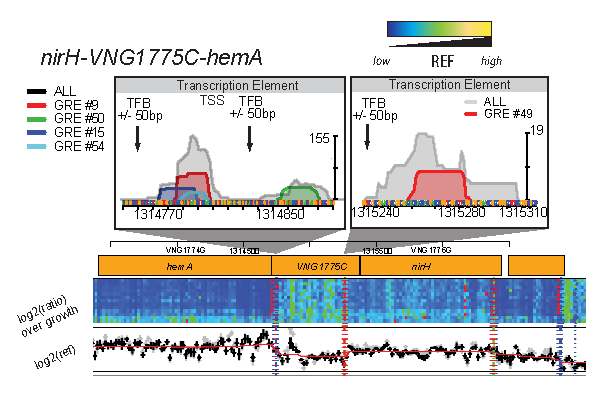
\includegraphics[width=0.6\linewidth]{figures/nirH.pdf}
\caption[GREs regulate multiple transcript isoforms from operons in {\it H. salinarum}, \textit{nirH-VNG1775C-hemA}.]{\textbf{GREs regulate multiple transcript isoforms from operons in {\it H. salinarum}, \textit{nirH-VNG1775C-hemA}.} GREs located inside operons coincide with experimentally measured transcriptional break sites. Experimentally determined transcription break sites (red dashed lines) above expression profiles of these regions across growth (heatmap, \cite{Koide2009} and ChIP-chip TFBs (\cite{Facciotti2007}, vertical arrows) support the role of GREs in regulating segmentation of the operon in certain conditions. Insets contain regions immediately surrounding transcriptional break sites, including counts of GREs discovered at these locations.}
\label{fig:nirH}
\end{figure}

\begin{figure}[h!]
\centering
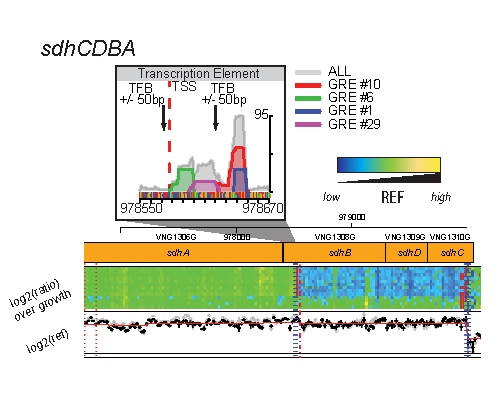
\includegraphics[width=0.6\linewidth]{figures/sdh.pdf}
\caption[GREs regulate multiple transcript isoforms from operons in {\it H. salinarum}, \textit{sdhCDBA}.]{\textbf{GREs regulate multiple transcript isoforms from operons in {\it H. salinarum}, \textit{sdhCDBA}.} Caption details included in Figure \ref{fig:nirH}}
\label{fig:sdh}
\end{figure}

\begin{figure}[h!]
\centering
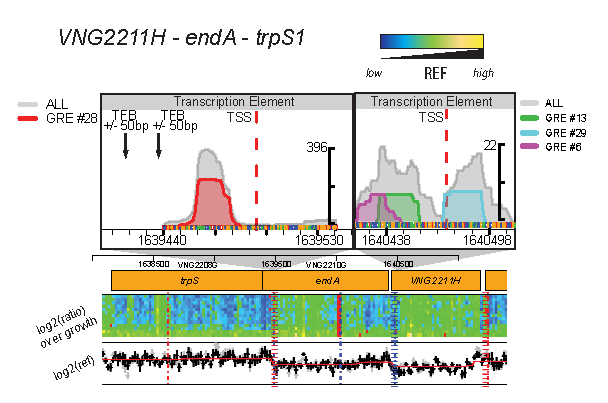
\includegraphics[width=0.6\linewidth]{figures/vng2211h.pdf}
\caption[GREs regulate multiple transcript isoforms from operons in {\it H. salinarum}, \textit{VNG2211H-endA-trpS1}.]{\textbf{GREs regulate multiple transcript isoforms from operons in {\it H. salinarum}, \textit{VNG2211H-endA-trpS1}.} Caption details included in Figure \ref{fig:nirH}}
\label{fig:vng2211h}
\end{figure}

\begin{figure}[h!]
\centering
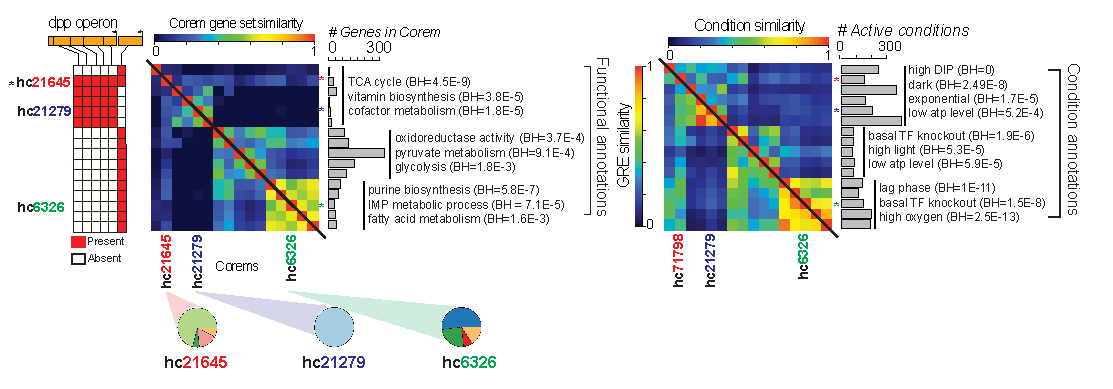
\includegraphics[width=0.95\linewidth]{figures/dpp_heatmaps.pdf}
\caption[Alternate regulatory modes for \textit{dpp} operon predicted by corems]{\textbf{Alternate regulatory modes for \textit{dpp} operon predicted by corems.} Corems group together functionally related sets of genes that are co-regulated in similar environments by similar factors (Left) Presence/absence of \textit{dpp} operon genes in corems. Three classes of corems exist for the dpp operon: (1) the entire operon (\eg hc21645), (2) the leader gene \textit{dppA} (\eg hc6326), and (3) five ``tail'' genes excluding \textit{dppA} (hc21279). (Middle) Gene similarity between corems (heatmap, Jaccard index). Functional annotations of genes in three highly similar clusters of corems to right. GRE composition for three corems shown below (pie chart, see Figure \ref{fig:corem_gres}). (Right) Similarity of conditions regulated (heatmap, upper triangle, Jaccard index) and GREs (heatmap, lower triangle, Jaccard index) among corems. Ordering is identical to (Middle). Environmental Ontology term enrichment (see ref{}) for three clusters depicted to right.}
\label{fig:dpp_heatmaps}
\end{figure}

\begin{figure}[h!]
\centering
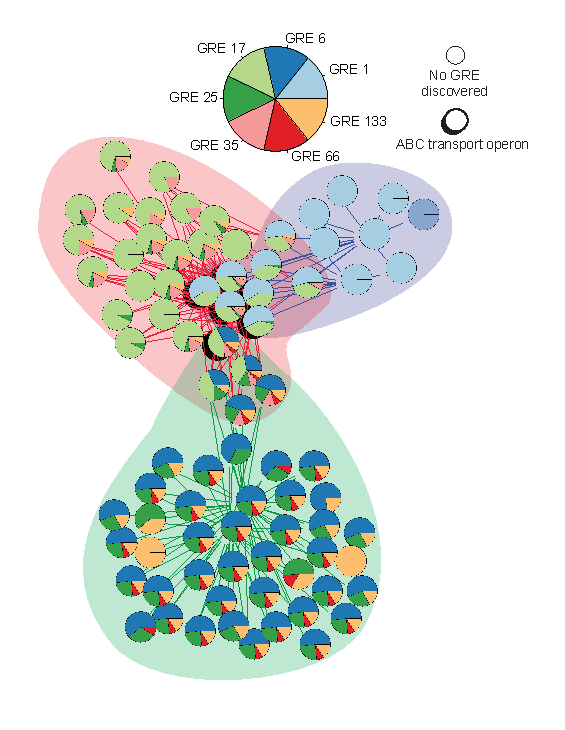
\includegraphics[width=0.6\linewidth]{figures/dpp_networks.pdf}
\caption[Network representation of transcriptional isoforms for the \textit{dpp} operon predicted by corems]{\textbf{Network representation of transcriptional isoforms for the \textit{dpp} operon predicted by corems.} Network representation for three corems described in \ref{fig:dpp_heatmaps}. Genes represented by circles. Edge colors and colored region behind the network indicate corem membership. Pie charts reflect GRE composition of each gene (see Figure \ref{fig:corem_gres}). Key for pie charts at top. Shading behind nodes (center of network) indicates \textit{dpp} operon genes.}
\label{fig:dpp_networks}
\end{figure}

\begin{figure}[h!]
\centering
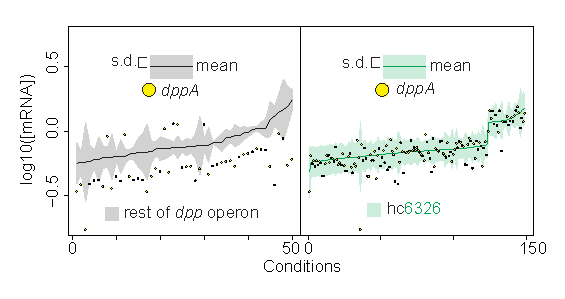
\includegraphics[width=0.6\linewidth]{figures/dpp_expression.pdf}
\caption[\textit{dppA} is more tightly co-expressed with genes of hc6326 in some environments than the other genes in the \textit{dpp} operon]{\textbf{\textit{dppA} is more tightly co-expressed with genes of hc6326 in some environments than the other genes in the \textit{dpp} operon.} Relative expression of \textit{dppA} compared to (left) other genes of \textit{dpp} operon and (right) hc6326.}
\label{fig:dpp_expression}
\end{figure}

\begin{figure}[h!]
\centering
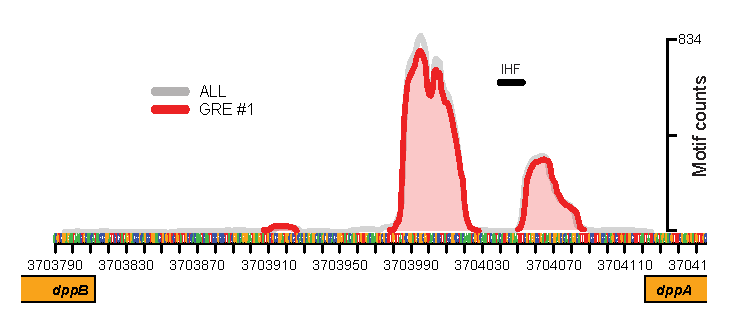
\includegraphics[width=0.6\linewidth]{figures/dpp_ecoli.pdf}
\caption[Evidence for condition-specific transcript isoforms of the \textit{dpp} operon in \textit{E. coli}]{\textbf{Evidence for condition-specific transcript isoforms of the \textit{dpp} operon in \textit{E. coli}.} \egrine~predicts conditional modulation of \textit{dpp} operon in {\it E. coli} as well. Promoter architecture within intergenic space between \textit{dppA} and \textit{dppB} suggested locations for TF binding internal to the operon (as in Figure 3A). GRE binding sites are proximal to an experimentally characterized IHF binding site (black horizontal bar; \rdb).}
\label{fig:dpp_ecoli}
\end{figure}

\begin{figure}[h!]
\centering
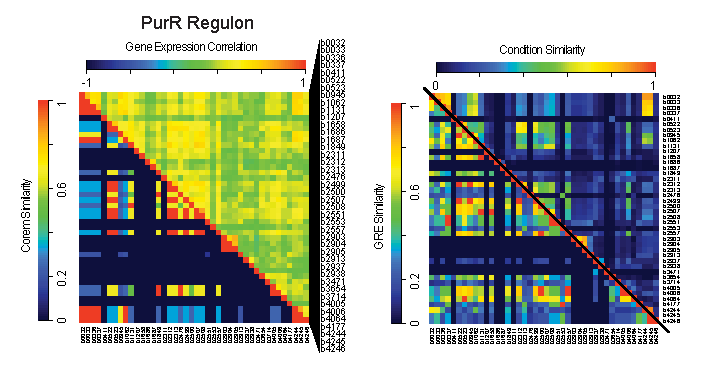
\includegraphics[width=0.95\linewidth]{figures/purR_heatmap.pdf}
\caption[Corems model the mechanistic basis for conditional subdivision of the PurR regulon, \textit{E. coli}]{\textbf{Corems model the mechanistic basis for conditional subdivision of the PurR regulon, \textit{E. coli}.} (Left) Corems identify the most highly correlated subgroupings of genes in PurR regulon. Gene expression correlation across all experiments (upper triangle) compared to similarity of corem membership (lower-triangle, Jaccard index) for genes of the PurR regulon (gene identifiers expanded to right). (Right) Similarity of regulated conditions (upper triangle, Jaccard index) and GREs composition for these genes (bottom triangle, Jaccard index). Consistent patterns of conditional-activity and GRE composition in their promoter regions further supports subdivision of PurR genes into separate corems. Gene order is same as left.}
\label{fig:purR_heatmap}
\end{figure}

\begin{figure}[h!]
\centering
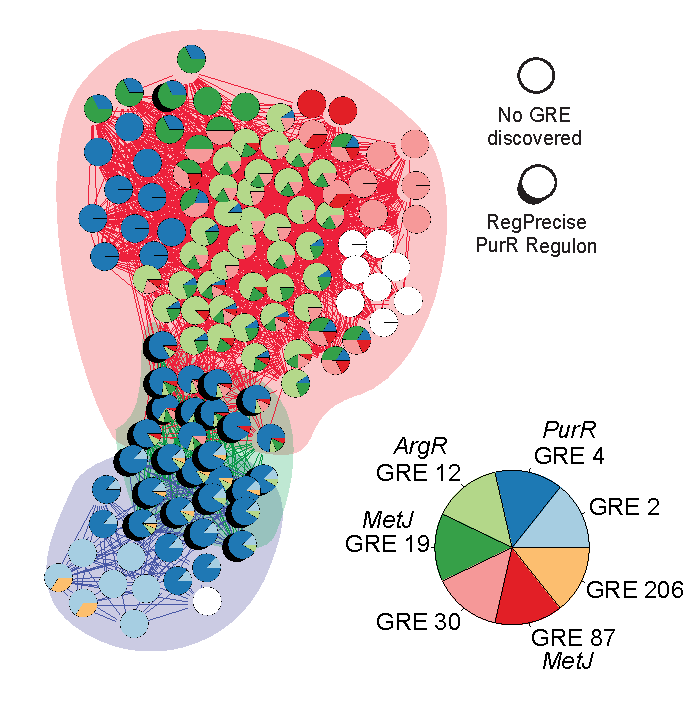
\includegraphics[width=0.6\linewidth]{figures/purR_network.pdf}
\caption[Corems integrate diverse regulatory mechanisms, \textit{E. coli}]{\textbf{Corems integrate diverse regulatory mechanisms, \textit{E. coli}.} Network representation for three corems described in Figure \ref{fig:purR_heatmap}. Genes are represented by circles. Edge colors and colored region behind the network indicate corem membership. Pie charts reflect GRE composition of each gene (see Figure~\ref{fig:corem_gres}). Key for pie charts at bottom. GRE-TF matches are indicated. Shading behind nodes denotes PurR regulon genes. At least 7 different mechanisms regulate the expression of these genes.}
\label{fig:purR_network}
\end{figure}


\begin{figure}[h!]
\centering
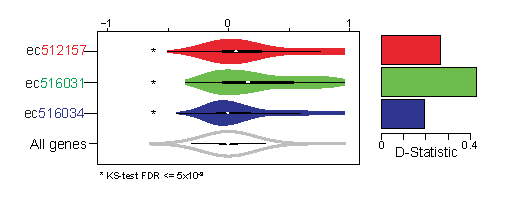
\includegraphics[width=0.7\linewidth]{figures/purR_corem_fitness.pdf}
\caption[Genes from corems related to nucleotide biosynthesis have highly similar fitness effects when they are deleted]{\textbf{Genes from corems related to nucleotide biosynthesis have highly similar fitness effects when they are deleted.} (Left) Violin plot shows distribution of all fitness correlations for genes in three nucleotide biosynthesis-associated corems compared to all genes in the data set. (Right) KS $D$-Statistic relates to enrichment for highly correlated gene-gene fitness associations in the corems. All three corems enrich for similar fitness effects (KS FDR $< 5\times 10^{-9}$)}
\label{fig:purR_corem_fitness}
\end{figure}

\begin{figure}[h!]
\centering
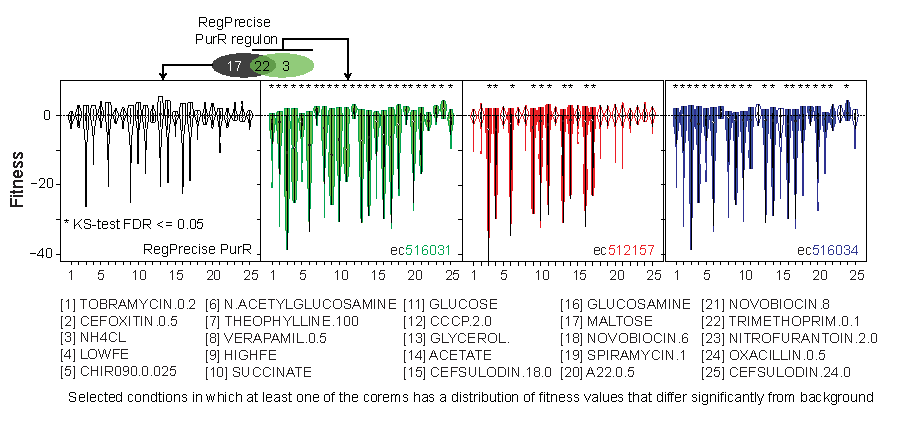
\includegraphics[width=0.95\linewidth]{figures/purR_corem_fitness_specific.pdf}
\caption[Corems model fitness effects that occur in specific environments]{\textbf{Corems model fitness effects that occur in specific environments.} Violin plots show distribution of relative fitness among corems across conditions (negative values indicate lower fitness relative to WT). Brief condition descriptions are displayed below. Shading within the violin plot indicates that the distribution of fitness values is significantly in that condition (KS-test FDR $\leq 0.05$). Fitness values for the subset of genes from the PurR regulon that do not occur in ec516031 are displayed to the left. These genes do not have significant fitness effects in any of the environments tested. Data from \cite{Nichols2011}.}
\label{fig:purR_corem_fitness_specific}
\end{figure}

\begin{figure}[h!]
\centering
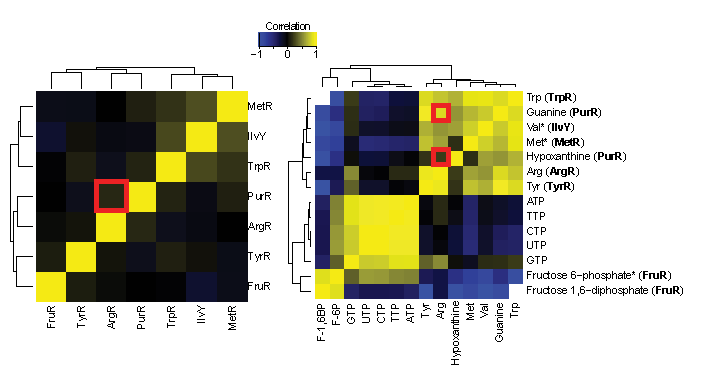
\includegraphics[width=0.95\linewidth]{figures/purR_effector.pdf}
\caption[Metabolite correlations may explain co-regulation within metabolically-linked corems]{\textbf{Metabolite correlations may explain co-regulation within metabolically-linked corems.} (Left) Expression correlation for TFs associated with three corems described in the text (ec516031,ec512157,ec516034). (Right) Correlation allosteric regulators for these TFs. TF regulated by each biomolecule listed in parentheses \cite{Novichkov2010}. Red boxes indicate PurR-ArgR and their corresponding effector molecules. Data from \cite{Ishii2007}.}
\label{fig:purR_effector}
\end{figure}

